%!TEX ROOT = ../presentation.tex


\section{First section name}% Section for TOC slides


\begin{frame}
    \vspace{9mm}
    Figure with the source of the image as footnote:\\
    % \vspace{3mm}
    \begin{figure}[H] \begin{center}
        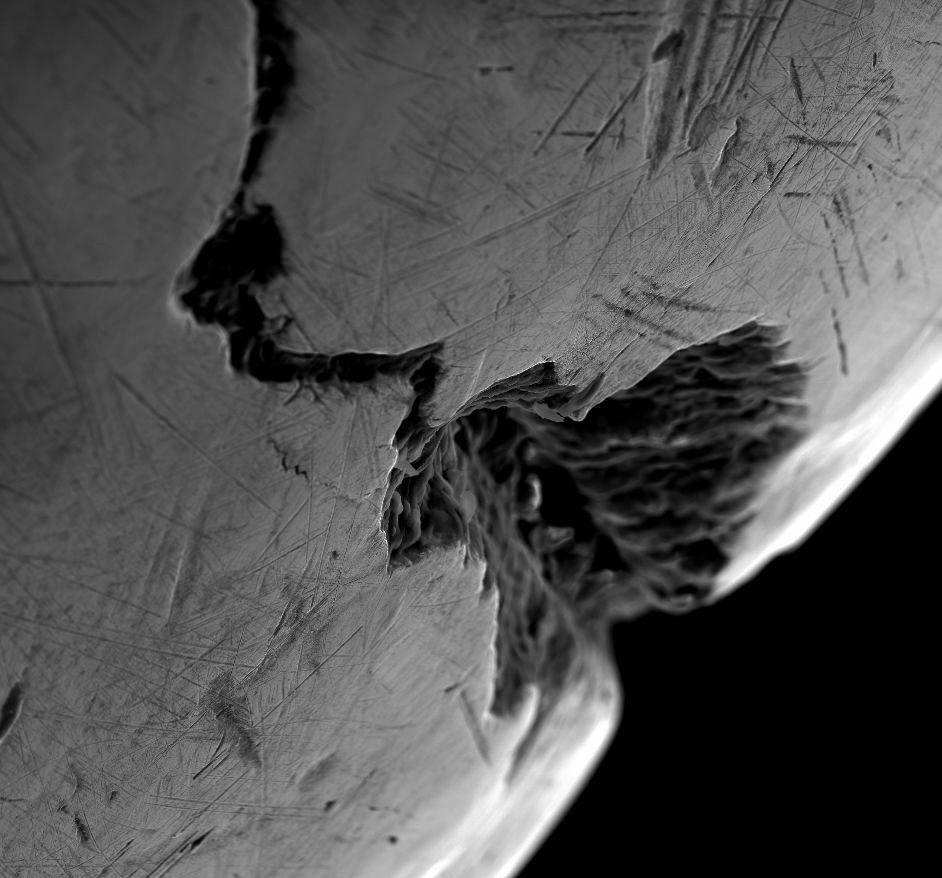
\includegraphics[height=0.7\textheight]{TitleImage_Crack}
    \end{center} \end{figure}
    \footn{Image source: Science \cite{ScienceCom}}
\end{frame}



\begin{frame}
    Side by side images from research by \cite{Web_Experiment}
    \begin{columns}
    \column{\dimexpr\paperwidth}
    \begin{figure}%
        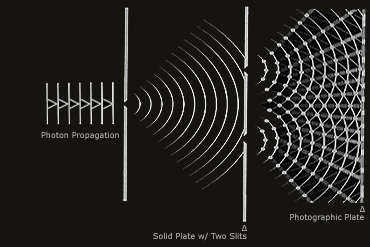
\includegraphics[height=0.4\textheight]{ExperimentalSetup}%
               \hspace{\dimexpr0.02\textwidth}%
        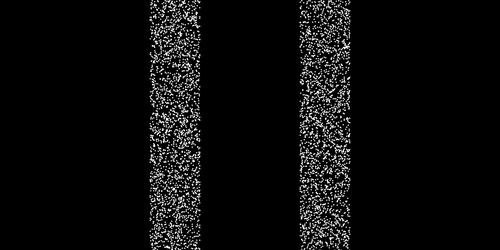
\includegraphics[height=0.4\textheight]{ExperimentalObservations}%
    \end{figure}%
    \end{columns}
    \footn{Source of images: theobservereffect.com \cite{Web_Experiment}}
\end{frame}



